\documentclass[runningheads]{llncs}
\usepackage[T1]{fontenc}
\usepackage{graphicx}
\usepackage{float}
\usepackage{color}
% uso de bibliografía
\usepackage[maxbibnames=99, style=numeric-comp, sorting=none, backend=bibtex]{biblatex}
\addbibresource{bibliografia/bibliografia.bib}
\addbibresource{bibliografia/creditriskprediction.bib}
\addbibresource{bibliografia/creditriskprediction_explainable.bib}
\addbibresource{bibliografia/reviews.bib}
\addbibresource{bibliografia/baseddecisiontree.bib}
\usepackage[colorlinks=true, urlcolor=blue, linkcolor=red, citecolor=green,]{hyperref}
\usepackage[english]{babel}
\usepackage{amsmath}
\usepackage[colorlinks=true, urlcolor=blue, linkcolor=red, citecolor=green]{hyperref}
\usepackage{caption}

\usepackage{tabularx}
\usepackage{booktabs}
\usepackage{array}
\begin{document}
	\title{An explainable algorithm for credit risk prediction based on contrast patterns}
	\author{Erwis Melchor Pérez\inst{1}\orcidID{0000-1111-2222-3333} \and
		José Francisco Martínez-Trinidad\inst{1}\orcidID{1111-2222-3333-4444} \and
		Jesús Ariel Carrasco Ochoa\inst{1}\orcidID{2222--3333-4444-5555}}
	
	\authorrunning{Melchor E. et al.}

	\institute{Instituto Nacional de Astrofísica, Óptica y Electrónica \email{\{emelchor,fmartine,ariel\}@inaoep.mx}}
	
	
	\maketitle
	\begin{abstract}
		Resumen
		\keywords{credit risk  \and pattern recognition \and clustering.}
	\end{abstract}
	
	\section{Introduction}\label{sec:introduction}
    Credit risk prediction involves determining whether an applicant will default on a future financial obligation \cite{zhu2025hybrid}, and is therefore a fundamental task in the financial sector. %In the literature, this topic is often referred to using different terms such as credit rating, credit scoring, loan evaluation, credit bond, and creditworthiness \cite{yeo2025comprehensive, lu2025llm, yu2025hybrid}. 
    Credit risk prediction is commonly considered as a supervised classification task; the goal is to assign each applicant to a class (e.g., default or non-default), rather than estimating a continuous predictive risk value. Credit risk prediction directly impacts the stability of banks and financial institutions, where accurate and explainable predictions are necessary to ensure regulatory compliance \cite{zhao2024improved, nguyen2025comparative}. Increasingly, financial institutions have implemented evaluations and management processes that employ pattern recognition and machine learning algorithms for credit risk prediction \cite{weber2024applications, yeo2025comprehensive}. As these predictors become more widely adopted, improving default prediction enables more accurate credit risk prediction and reduces losses \cite{lu2025llm, hartomo2025novel, yu2025hybrid}.\\

    Recent research in credit risk prediction has prioritized improving the performance of credit risk prediction algorithms based on machine learning and pattern recognition through the use of oversampling or undersampling methods, thereby reducing algorithmic bias towards the majority class \cite{adiputra2025effectiveness, ali2025explainable, kandi2025enhancing, darwish2025intelligent, hu2025combining}; the use of feature selection methods for identifying the most relevant features of a dataset to improve the performance of prediction algorithms \cite{zhu2025hybrid, gasmi2025features, zou2025variable, wang2024feature}; and the use of explainable AI techniques \cite{ali2025explainable, lin2025credit, zhang2025method, han2024nate} that allow users to comprehend and trust the predictions provided by credit risk prediction algorithms, which makes the predictions of the algorithm to comply with regulations.\\
        
    Machine learning algorithms have demonstrated good predictive performance, and decision trees are among the most effective for credit risk prediction \cite{weber2024applications, chang2024prediction, aruleba2024effective, zhang2025blockchain, xia2025confidence, wu2024credit, zou2025interpretable}. However, the need for explanations remains a significant limitation, particularly in the financial sector, as financial institutions and regulators require justification for their decisions \cite{sowmiya2024credit, ravi2025explainable}. Several authors have addressed the lack of explainability in credit risk prediction \cite{lin2025credit, zandi2025attention,sun2025enhancing}. \newline
    
    Explainability techniques, also known as XAI (eXplainable Artificial Intelligence), aim to make machine learning prediction processes transparent and understandable to humans. These techniques are important in areas such as credit risk prediction, where justifying and explaining the predictions is essential in enabling financial institutions to make more informed decisions. Several recent studies have applied SHAP \cite{lundberg2017unified} and LIME \cite{ribeiro2016should} to credit risk prediction to generate explanations for individual predictions \cite{garcia2025machine, baisholan2025fraudx, alonso2025should}. SHAP assigns to each feature a value that represents how much it contributed to the prediction. These values help explain the role each feature played in the prediction. LIME builds a simple interpretable predictor that approximates the behaviour of the original predictor by modifying a specific instance and observing the changes in the prediction. The result is an explanation that highlights the features contributing most to the prediction, showing how each affects the prediction in a positive or negative direction. However, these techniques focus on individual features and often overlook how several features jointly contribute to the prediction. \\

    In credit risk prediction, a predictor's output depends on multiple features rather than individual features. Therefore, explainable predictors should consider multiple features to explain the prediction \cite{zhang2025method, do2024explainable}. In response to this need, this paper proposes a credit risk prediction algorithm that generates explanations based on contrast patterns, which are conjunctions of conditions of the form $feature \# value$ that are frequent in a class but rarely appear in the opposite class. Since contrast patterns can be extracted from decision-tree-based, we propose using decision-tree-based predictors to predict credit risk, which have been reported  to perform competitively compared to the most successful approaches. In this way, the proposed algorithm leverages the affinity and synergy between decision-tree-based predictors, and contrast patterns extracted from decision treed. \newline
    
    Unlike other explainable algorithms that merely highlight the importance of individual features, our method explains predictions based on contrast patterns present in the training data and shared with the new applicant. Experiments conducted on both public and private financial datasets show that the proposed algorithm achieves competitive predictive accuracy while offering instance-level explanations based on the contrast patterns shared with other clients in the class, unlike the current state-of-the-art, which explains based on the single features contributing most to the prediction.\\
	
    %The remainder of this paper is organized as follows. Section \ref{sec:relatedworks} presents the related work. Section \ref{sec:explainablealgorithm} describes the proposed algorithm. Section \ref{sec:experimentsresults} presents the experimental results. Finally, Section \ref{suc:conclusion} presents our conclusions and future work directions.
    The remainder of this paper is organized as follows. Section 2 presents the related work. Section 3 describes the proposed algorithm. Section 4 presents our experimental results and a discussion about them. Finally, Section 5 presents our conclusions and future work directions.
    
	\section{Related works}\label{sec:relatedworks}
    Credit risk prediction has been extensively studied in the literature using a wide range of pattern recognition and machine learning algorithms \cite{gasmi2025features, bai2025improved, dougan2025credit, aruleba2025improved, yao2025novel, liang2025application, lu2025efficient, yu2025hybrid, nguyen2025comparative, zou2025variable, zeng2025nexus, hartomo2025novel, ali2025explainable, zandi2025attention, sun2025enhancing, zhou2025enhancing, baisholan2025fraudx, oliveira2025advancing, lin2025deep, sundaravadivel2025optimizing, kandi2025evaluating, wang2025two}. %nobel2024unmasking, do2024explainable, zhao2024resampling, chang2024credit, zhuang2024design, talaat2024toward, mosa2024ccfd, pavitha2024explainable, jacobs2024benchmarking, chen2024interpretable, nallakaruppan2024credit, alblooshi2024unlocking, mienye2023deep, bakhtiari2023credit, gao2023cate, de2022explainable, moscato2021benchmark, ariza2020explainability
    In this section, we review the most recent works on credit risk prediction, with a focus on approaches that either prioritize achieving the highest accurate credit risk prediction or incorporate explainability for credit risk prediction. The works considered in this review are those that utilize publicly available datasets, commonly used in the literature and accessible online, which allows a comparison against our proposal. Accordingly, this section is divided into two parts: works that focus solely on accuracy without offering explanations, and works that integrate explainability into their predictors.
    \subsection{Predictors for Credit Risk Prediction}

    Recent works on credit risk prediction have focused on developing predictive algorithms to improve performance metrics, such as accuracy, area under the curve (AUC), Type II error, or F1-score.\\
    
    % Primero empezaré con aquellos que no explican pero tiene buenos resultados
    % aruleba2025improved este trabajan con german y australian
    In \cite{aruleba2025improved}, the authors proposed a stacked ensemble for credit risk prediction that combines Random Forests (RF), Logistic Regression (LR), and Convolutional Neural Networks (CNN). The results of these predictors are used as input features for a Multilayer Perceptron (MLP), which learns to combine them to produce the prediction. The authors used SMOTEENN \cite{batista2004study} to address class imbalance, and the stacked ensemble is compared against CNN, LR, MLP, and RF. After applying SMOTE-ENN to address class imbalance, the stacked ensemble consistently outperformed the individual predictors, achieving accuracies near 96\%.\\ 
    
    A comparative study of different predictors for credit risk prediction is presented in \cite{sundaravadivel2025optimizing}, including LR, RF, and Artificial Neural Networks (ANN). In this study, SMOTE \cite{chawla2002smote} was employed to balance the training dataset, leading to significant improvements in the performance metrics of all predictors. Among them, RF achieved the best results, with an accuracy of 98\%.\\

    In \cite{kandi2025evaluating}, Deep Convolutional Neural Networks (DCNN) and Support Vector Regression (SVR) were compared for credit risk prediction. The application of SMOTE contributed to improved predictive performance in both predictors. Using SMOTE to balance the dataset, SVR achieved an accuracy of 98\% and F1-score of 87\%.\\
    
    In \cite{zou2025level}, the authors present the Level-Wise Feature-Guided Cascading Ensembles (LFGCE) model, which integrates hierarchical feature selection with a cascading ensemble learning scheme. To evaluate its performance, several predictors were employed, including RF, Support Vector Machines (SVM), LR, Decision Trees (DT), ANN, Linear Discriminant Analysis (LDA), and XGBoost. Among these, XGBoost achieved the best results in both feature selection and prediction, with an AUC of 94\%. However, it is important to note that the study does not address class imbalance, as no data balancing methods were applied.\\ 

    Most of the reviewed studies emphasise improving predictive performance through class balancing methods to mitigate data imbalance. Several predictors yield good results in credit risk prediction. However, the reported performance metrics (such as accuracy, AUC, and F1-score) vary significantly on the chosen predictors and balancing methods. Overall, the authors consistently point out that addressing class imbalance is crucial for achieving reliable predictions, with many studies reporting high accuracy values, often exceeding 90\%. %, tree-based predictors such as Random Forests and XGBoost achieve the best results.


    \subsection{Explainable Predictors for Credit Risk Prediction}

    Incorporating explainability into credit risk prediction has been a growing area of study. These studies aim to achieve robust predictive performance while prioritising the explainability of predictions.\\

    A study by \cite{zhou2025enhancing} addresses credit risk prediction by comparing the predictive performance of XGBoost, RF, Least Squares SVM (LSSVM), and a CNN. After applying SMOTE to balance the dataset, XGBoost achieved the best predictive accuracy, reaching 92\%. To enhance predictor explainability, SHAP analysis was applied to quantify the individual contributions of each feature. From the predictors evaluated, XGBoost performed best in terms of predictive accuracy and also provided explanations through SHAP values.\\ 

    In \cite{baisholan2025fraudx}, the authors present an ensemble framework that combines RF and XGBoost using probability-weighted averaging. The framework was evaluated using eight predictors, including LR, DT, Gradient Boosting (GB), LightGBM (LGBM), MLP, Naive Bayes (NB), and XGBoost. Their proposed ensemble significantly outperformed all others, achieving an AUC of 97\%. SHAP was employed to explain the predictions, which allowed them to determine the contribution of each feature.\\

   In \cite{sun2025enhancing}, XGBoost is used as a predictor, combined with SHAP, LIME, and K-means to enhance explainability, achieving an AUC of 78\%. SHAP and LIME are used to generate feature-contribution vectors for each training instance, which are grouped using K-means. For explaining the prediction of a new instance, its feature-contribution vector is calculated and assigned to the nearest cluster, and the prediction explanation is provided as the cluster’s average vector.\\

    In \cite{nguyen2025comparative}, the authors present a comparative analysis of the performance of boosting algorithms, including LightGBM, XGBoost, CatBoost, and AdaBoost. Additionally, SMOTE-Tomek \cite{batista2003balancing} is employed to balance the dataset. The results indicate that LightGBM achieves the best performance with 95\%  accuracy and 98\% AUC, outperforming the other boosting methods. SHAP is applied to quantify the contribution of each feature to the prediction.\\

    In \cite{zandi2025attention}, a multilayer dynamic graph neural network (DYMGNN), proposed for credit risk prediction. The authors compare their approach against several baselines: LR, XGBoost, and DNN. Unlike many related studies, no resampling or class balancing methods are applied. Experimental results show that the DYMGNN achieves the best results with 81\% accuracy and 83\% F1-score. For explainability, SHAP is used to identify the features that contribute most to the predictions. \\

    In \cite{wang2025two}, the authors propose an explainable two-stage technique to explain the results of credit risk prediction. In the first stage, SHAP is applied to analyse the importance of features according to their positive or negative impact on the prediction. In the second stage, they use a genetic algorithm to generate counterfactual explanations by perturbing the features according to this categorisation, thereby identifying the minimum necessary changes to modify the prediction. This technique was evaluated using multiple predictors, including SVM, XGBoost, MLP, and LSTM, with an accuracy of 90\% for the employed predictors. The results demonstrate that the features modified most frequently closely align with the features identified as most relevant by SHAP.\\

    In \cite{aruleba2025enhanced}, the authors compare the performance of several Deep Learning (DL) architectures for credit risk prediction, including Convolutional Neural Networks (CNN), Long Short-Term Memory (LSTM) networks, Gated Recurrent Units (GRU), and Graph Neural Networks (GNN). To address class imbalance, they apply SMOTEENN. The experimental results show that GRU outperformed all other predictors, achieving an accuracy of 91\%. To explain the prediction, SHAP is used to quantify the importance of features and their contributions to the predictions.\\

    In \cite{hartomo2025novel}, the authors propose an approach for credit risk prediction on imbalanced datasets by integrating the TabTransformer model with a weighted loss function. This approach helps mitigate the bias toward the majority class, improving predictive performance on minority classes, achieving 91\% accuracy and an AUC of 93\%. SHAP is employed to evaluate feature importance and identify those features that contribute most to the predictions.\\
    
    In \cite{damanik2025advanced}, the authors propose a robust framework for credit risk prediction on imbalanced datasets by introducing the K-SMOTEENN method, which integrates oversampling and noise-filtering methods with a stacking ensemble. The ensemble combines Random Forest, XGBoost, and LightGBM, resulting in a predictive performance of 92\% F1-score, and 96\% AUC. SHAP is used to analyse and explain the contributions of individual features to the prediction.\\
    
    %In \cite{han2024nate}, the authors propose NATE, a non-parametric approach to credit risk prediction in imbalanced datasets that integrates GB as a predictor. The study compares GB with other classifiers, including LR, SVM, XGBoost, and RF, demonstrating that GB achieves the highest predictive performance with an AUC of 96\% and a F1-score of 90\%. NATE applies SMOTE to balance the dataset and employs SHAP to explain the prediction, highlighting the contribution of each feature to the prediction.\\ 

    %In \cite{talaat2024toward}, the authors propose CreditNetXAI, which combines deep neural networks with XAI techniques for credit risk prediction, using feature selection methods to identify the most relevant features for prediction. CreditNetXAI obtains an accuracy of 83\%. To explain predictions, they use SHAP to assign an importance to each feature and indicate its contribution to the prediction.\\ 

    %In \cite{zheng2024micro}, the authors employ Decision Tree-based LightGBM with an optimized gradient approach to credit risk prediction, demonstrating an accuracy of 93\% and an AUC of 80\%.  To explain the prediction, they use SHAP to show the importance of features in the prediction. Similarly in \cite{de2022explainable} used a LightGBM for credit risk prediction, achieving an accuracy of 82\% and SHAP to explain the prediction. In \cite{nallakaruppan2024explainable}, the authors propose using RF with explainable AI techniques for credit risk prediction, achieving an accuracy of 99\%. To generate explanations for predictions, LIME, SHAP, and Partial Dependence Plots (PDPs) were used, which help identify how feature values contribute to the prediction. It is important to note that these results were obtained on different datasets, making direct comparison between reported accuracies and AUCs not the same. \\

    As discussed in the above works, credit risk prediction has been addressed through a wide range of predictors, balancing methods, feature selection methods, and evaluated through multiple performance metrics. Nevertheless, accurately detecting defaults remains a significant challenge, as no single method has consistently outperformed others across different scenarios. Moreover, the most commonly used explainability approaches, such as SHAP and LIME, while helpful in assessing the individual contribution of features, fail to capture feature value combinations that characterise different types of applicants. This limitation is particularly relevant, since financial institutions increasingly demand not only high predictive accuracy but also clear and case-specific justifications, both to meet regulatory requirements and to improve communication with applicants. 
    
    
	\section{Proposed explainable algorithm}\label{sec:explainablealgorithm}
% Boran Tae 
        As discussed in the previous section, recent research has increasingly focused on explaining credit risk predictions. Techniques such as SHAP and LIME, commonly used for explaining credit risk predictions, assign importance scores to individual features; however, they do not capture the joint effect of multiple features in a prediction, which is particularly relevant in credit risk prediction. This limitation highlights the need for approaches that go beyond individual feature contributions and consider multiple features when explaining credit risk predictions.\newline

    	The idea behind the proposed Pattern-based Credit Risk Prediction and Explanation (PbCRPE) algorithm is to enable both credit risk prediction and its explanation to rely on the same approach. Unlike traditional explainers for credit risk prediction, which apply a predictor that follows an approach different from the one used for explaining predictions (e.g., SHAP or LIME which are commonly based on individual feature contribution techniques), PbCRPE predicts and explains following a similar approach.\newline
    	
    	As mentioned previously, credit risk prediction depends on multiple features rather than individual features. For instance, a 'high debt-to-income ratio' may only indicate default when combined with 'low job stability'. This observation highlights the need for explanation approaches that consider multiple features. In this context, PbCRPE addresses this need by using contrast patterns to explain predictions. Contrast patterns allow providing explanations based on conjunctions of $feature\#value$ conditions, similar to those used by decision trees. This structural similarity motivates the use of a predictor based on decision trees, not only because of their alignment with contrast patterns, but also because of their strong performance in state-of-the-art credit risk prediction \cite{aruleba2025improved}. A decision tree can be interpreted as a hierarchy of decision rules, where each path from the root to a leaf node corresponds to a conjunction of conditions of the form $feature\#value$. Similarly, contrast patterns are expressed as conjunctions of conditions of the form $feature\#value$. Based on this relationship, the proposed algorithm is organized into two main stages: (i) a training stage, which includes predictor training and contrast pattern mining from the classes, and (ii) a prediction and explanation stage using the trained predictor and the mined contrast patterns.

		\subsection{Training and contrast pattern mining stage}
		{\color{blue}
			The first stage of the PbCRPE consists of training a classifier for a credit risk predictor and mining contrast patterns, which are expressed as a conjunction of $feature\#value$ conditions that will later be used to explain the classifier's predictions. \newline 
		}
		
		For credit risk prediction, we propose using the FT4cip predictor \cite{canete2022ft4cip}, a decision tree-based predictor capable of handling mixed and imbalanced datasets, which has reported strong predictive quality on such data, making it suitable for this task. Although FT4cip is designed to handle imbalanced datasets, the experiments conducted in this work indicated that it achieved better predictive quality when trained using a previously balanced training set. Thus, following the results reported in \cite{melchor2025oversampling}, we propose applying SMOTENC \cite{chawla2002smote, mukherjee2021smote} to the training set to balance it prior to predictor training.\newline
		
		{\color{blue}	
		For mining contrast patterns, since instances belonging to the same class do not necessarily share the same $feature\#value$ groups of similar instances are first identified through clustering. Contrast patterns are subsequently mined independently for each cluster with respect to the whole opposite class, yielding contrast patterns that characterize instances in the class specific to both the cluster and its associated class. To generate these clusters, we propose using the Kmodes algorithm \cite{huang1997clustering, huang1998extensions}, as it is specifically designed for mixed data and avoids the limitations of distance-based methods when handling non-numeric features. To determine the number of clusters, following \cite{dinh2019estimating, kuswardana2025comparison}, we propose using the Silhouette coefficient, which, according to these works, enables the identification of well-defined clusters. 
		}\newline 
		
		For mining contrast patterns, we propose using CPMining, introduced in the PBC4cip algorithm \cite{garcia2010lcmine, loyola2017pbc4cip}, as a supervised contrast pattern miner that explicitly exploits class differences to identify contrast patterns. CPMining is applied independently to each cluster by contrasting the instances of the cluster with all instances of the opposite class. This design allows mining contrast patterns that represent $feature\#value$ conditions observed among similar instances within each cluster while appearing less in instances from the opposite class.\newline
		
		Due to the large number of contrast patterns that can be generated during mining, the filtering used in CPMining is applied to reduce redundant patterns. This filtering removes more specific patterns when a more general pattern covers the same instances, and when redundant conditions are present within a pattern. Additionally, we propose removing contrast patterns whose support in the opposite class is non-zero. As a result, the final set contains only contrast patterns whose support in the opposite class is zero.
		
       \subsection{Prediction and explanation stage}
       
       Given a new instance $x$, the prediction and explanation stage first determines its class (defaulter or non-defaulter) using the trained FT4cip predictor. Once the predicted class $c$ for $x$ has been determined, the contrast patterns mined from each cluster associated with class $c$ are used to compute a similarity score between the new instance $x$ and each cluster. The cluster with the highest similarity score is selected as the cluster most similar to the new instance. \newline %A contrast pattern selected from this cluster constitutes the explanation of the prediction. \newline
       
       To identify the cluster that best represents a new instance $x$, PbCRPE defines a contrast pattern-based similarity score between $x$ and each cluster $C_{c,j}$ associated with the predicted class $c$. Unlike conventional similarity measures for mixed data, which compare instances directly using their feature values, the proposed score evaluates similarity through the contrast patterns mined from each cluster. These patterns summarize the characteristic combinations of $feature\#value$ conditions shared by similar instances within the cluster and associated with the predicted class, making them a more appropriate representation for explanation purposes. Consequently, the similarity between $x$ and a cluster is quantified according to the support accumulated by the cluster's contrast patterns that cover the new instance. Specifically, the similarity score is computed as the ratio between the accumulated support of the covering contrast patterns and the total support of all contrast patterns mined from the cluster, as defined in Equation~\ref{eq:cluster_similarity}.\newline
             
       \begin{equation}
       	Sim(x, C_{c,j})
       	=
       	\frac{
       		\sum\limits_{p \in \mathcal{P}_{c,j}(x)} supp(p)
       	}{
       		\sum\limits_{p \in \mathcal{P}_{c,j}} supp(p)
       	},
       	\label{eq:cluster_similarity}
       \end{equation}
       
       This similarity score increases as the support of the contrast patterns covering the new instance increases. Since contrast patterns with higher support cover more similar instances within the cluster, they contribute more to the similarity score. Furthermore, dividing by the total support of the contrast patterns mined from the cluster avoids bias towards clusters with more contrast patterns. Consequently, higher similarity scores indicate that a larger proportion of the support of the contrast patterns mined from the cluster is associated with to contrast patterns that cover the new instance.\newline
       
{\color{blue}		       
		The cluster with the highest similarity score is selected as the cluster most similar to the new instance $x$. If multiple clusters obtain the same highest similarity score, the cluster whose highest-support contrast pattern covering the new instance has the greatest support is selected. If a tie persists, the cluster whose corresponding highest-support contrast pattern contains the largest number of $feature\#value$ conditions is selected. This tie-breaking criterion favors the cluster whose covering contrast pattern has the greatest support and, when support is equal, provides the most specific combination of conditions. The explanation stage assumes that at least one contrast pattern mined from the clusters associated with the predicted class covers the new instance. Under this assumption, empirically validated later a Section \ref{sec:experimental}the most similar cluster always contains at least one covering contrast pattern. Once the most similar cluster $C_{c,j^*}$ has been identified, the contrast pattern $p^*$ with the highest support is selected from $\mathcal{P}_{c,j^*}(x)$, the set of contrast patterns from $C_{c,j^*}$ that cover the instance $x$, as defined in Equation~\ref{eq:pattern_selection}. Support is used as the selection criterion because contrast patterns with higher support cover a larger number of similar instances within the selected cluster, indicating that more instances share the same $feature\#value$ conditions.
	}
       
       \begin{equation}
       	p^* = \arg\max_{p \in \mathcal{P}_{c,j^*}(x)} supp(p),
       	\label{eq:pattern_selection}
       \end{equation}
       
		The selected contrast pattern becomes the final explanation of the prediction and is expressed as a conjunction of $feature\#value$ conditions. Since the selected contrast pattern covers multiple similar instances within the most similar cluster, the explanation is based on conditions shared by the new instance and those covered instances. If multiple patterns achieve the same maximum support, the pattern containing the largest number of $feature\#value$ conditions is selected, since it provides a more detailed explanation by incorporating a larger set of conditions associated with the covered instances. If multiple contrast patterns remain tied after applying this criterion, all tied contrast patterns will be the explanation. \\
		
		Unlike recent works, where explainability highlights individual features that contribute most to the prediction, showing how each affects the prediction in a positive or negative direction. In our proposal, explainability involves several features that jointly contribute to the prediction.
       

	%waiting for a girl like you
{\color{blue}
\section{Experimental Results}\label{sec:experimental}
The objective of this experimental evaluation is to assess whether PbCRPE can achieve competitive credit risk prediction quality compared with other state-of-the-art works while simultaneously providing explainable predictions based on combinations of multiple features that jointly contribute to the prediction. The evaluation considers two complementary aspects of prediction quality, assessed using AUC and Type~II Error, two commonly used metrics in credit risk prediction that capture different aspects of predictive quality: the overall ability of the predictor to discriminate between defaulters and non-defaulters and its ability to correctly identify defaulters, respectively. While a competitive AUC indicates that PbCRPE maintains a strong overall discrimination capability, particular emphasis is placed on Type~II Error because incorrectly classifying a defaulter as a non-defaulter may result in direct financial losses for lending institutions. Therefore, achieving a low Type~II Error is particularly relevant from a practical credit risk perspective, and the experimental evaluation investigates whether PbCRPE can provide an advantage in this aspect while maintaining competitive overall prediction quality.\newline

PbCRPE is compared with twelve recent state-of-the-art credit risk prediction works using the same experimental setup and twelve public and private credit risk datasets. These works were selected from studies published between 2024 and 2025 because they represent recent developments in machine-learning-based and explainable credit risk prediction, report competitive prediction results, and evaluate their algorithms on benchmark datasets that overlap with or are comparable to those considered in this work. The results show that PbCRPE achieves competitive prediction quality in terms of AUC compared with the evaluated state-of-the-art works, while obtaining the best overall result in terms of Type~II Error. This result is particularly relevant from a practical perspective because a lower Type~II Error indicates a lower proportion of actual defaulters incorrectly classified as non-defaulters. Therefore, the experimental evaluation shows that PbCRPE maintains competitive overall prediction quality while achieving a particular advantage in identifying actual defaulters and reducing the risk of incorrectly classifying them as non-defaulters.

\subsection{Datasets}

The experimental evaluation was conducted using twelve credit risk datasets obtained from both public and private sources. The datasets were selected because they represent diverse credit risk scenarios while sharing the two characteristics addressed by the proposed PbCRPE algorithm: mixed-type data, including numerical and categorical features, and different degrees of class imbalance. The diversity in feature types and class distributions allows the prediction quality of PbCRPE to be evaluated under different data conditions.\newline

Table~\ref{conjuntodedatos} summarizes the main characteristics of the datasets, including the number of instances, number of features (total, numerical, and categorical), class distribution, imbalance ratio (IR), and data source. The eleven public datasets were obtained from the UCI Machine Learning Repository\footnote{\url{https://archive.ics.uci.edu/}} and Kaggle\footnote{\url{https://www.kaggle.com/}}, two widely used repositories for benchmarking credit risk prediction algorithms. The twelfth dataset was provided by a private financial institution. Due to a confidentiality agreement, the identity of the institution and further information about the dataset cannot be disclosed. The datasets vary substantially in both size and class distribution, ranging from 628 to 150,000 instances and from nearly balanced datasets (IR = 1.09) to highly imbalanced datasets (IR = 13.96). Consequently, the experimental evaluation covers a broad spectrum of credit risk scenarios, allowing the prediction quality of PbCRPE to be assessed under different levels of class imbalance.
	\begin{table}[H]
		\centering
		\caption{Characteristics of the twelve credit risk datasets used in the experimental evaluation.}
		\label{conjuntodedatos}
		\resizebox{12cm}{!}{%
			\begin{tabular}{lccccccc}
				\hline
				\multicolumn{1}{c}{\textbf{Dataset}} &
				\textbf{Instances} & \textbf{Features} &
				\textbf{Numerical/Categorical} &
				\textbf{No-defaulter} & \textbf{Defaulter} &
				\textbf{IR} & \textbf{Domain} \\ \hline
				AER            &   1,319   & 12 & 9/3   &   1,023  &    296  &  3.45  & Public  \\
				Australia      &     690   & 14 & 6/8   &     307  &    383  &  1.24  & Public  \\
				Japan          &     690   & 15 & 6/9   &     307  &    383  &  1.24  & Public  \\
				EIZ            &   5,510   & 22 & 13/9  &   2,295  &  3,215  &  1.40  & Private \\
				German         &   1,000   & 20 & 7/13  &     700  &    300  &  2.33  & Public  \\
				HMEQ-Data      &   3,364   & 12 & 10/2  &   3,064  &    300  & 10.21  & Public  \\
				Taiwan         &  30,000   & 24 & 20/3  &  23,364  &  6,636  &  3.52  & Public  \\ % corrected: 30,000
				GMSC           & 150,000   & 11 & 10/1  & 139,974  & 10,026  & 13.96  & Public  \\
				Heloc          &  10,459   & 23 & 23/0  &   5,000  &  5,459  &  1.09  & Public  \\
				Loan data set  &     628   & 12 & 7/4   &     332  &    296  &  1.12  & Public  \\
				PPDai          &  55,596   & 29 & 22/7  &  48,413  &  7,183  &  6.74  & Public  \\
				Thomas dataset &   1,225   & 14 & 14/0  &     902  &    323  &  2.79  & Public  \\
				\hline
		\end{tabular}}
	\end{table}
\subsection{Credit risk prediction quality}

Figures~\ref{fig:rocauc} and~\ref{fig:type2} compare the prediction quality of PbCRPE with that of the twelve selected state-of-the-art approaches using AUC and Type~II Error, respectively. For each dataset, a stratified 5-fold cross-validation procedure was employed, in which the data were divided into five folds while preserving the class distribution across folds. In each iteration, four folds (approximately 80\% of the instances) were used for training and the remaining fold (approximately 20\%) was used for testing. The process was repeated five times, with each fold serving once as the test set. The same cross-validation protocol was applied to PbCRPE and all compared approaches to ensure a fair and consistent evaluation. The reported AUC and Type~II Error values correspond to the mean results obtained across the five folds. Figure~\ref{fig:rocauc} reports the mean AUC across the twelve evaluated datasets, whereas Figure~\ref{fig:type2} presents the corresponding mean Type~II Error across the same datasets.\newline

\begin{figure}[H]
	\centering
	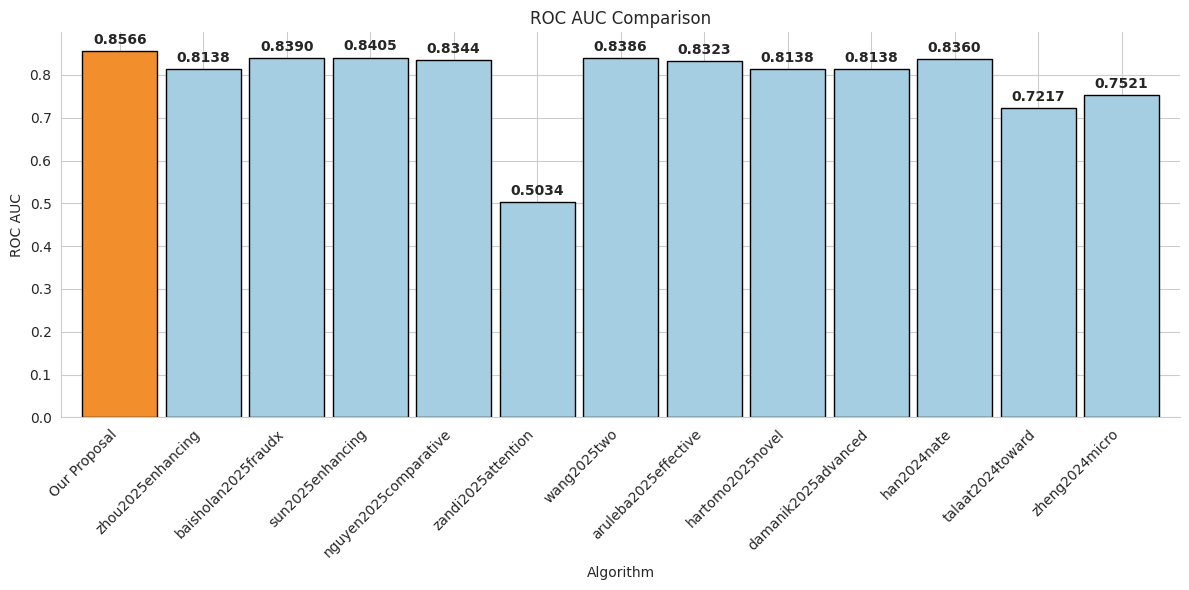
\includegraphics[width=0.9\linewidth]{img/rocauc}
	\caption{Mean AUC obtained by PbCRPE and the compared state-of-the-art approaches across the twelve evaluated credit risk datasets. Higher values indicate better prediction quality.}
	\label{fig:rocauc}
\end{figure}

\begin{figure}[H]
	\centering
	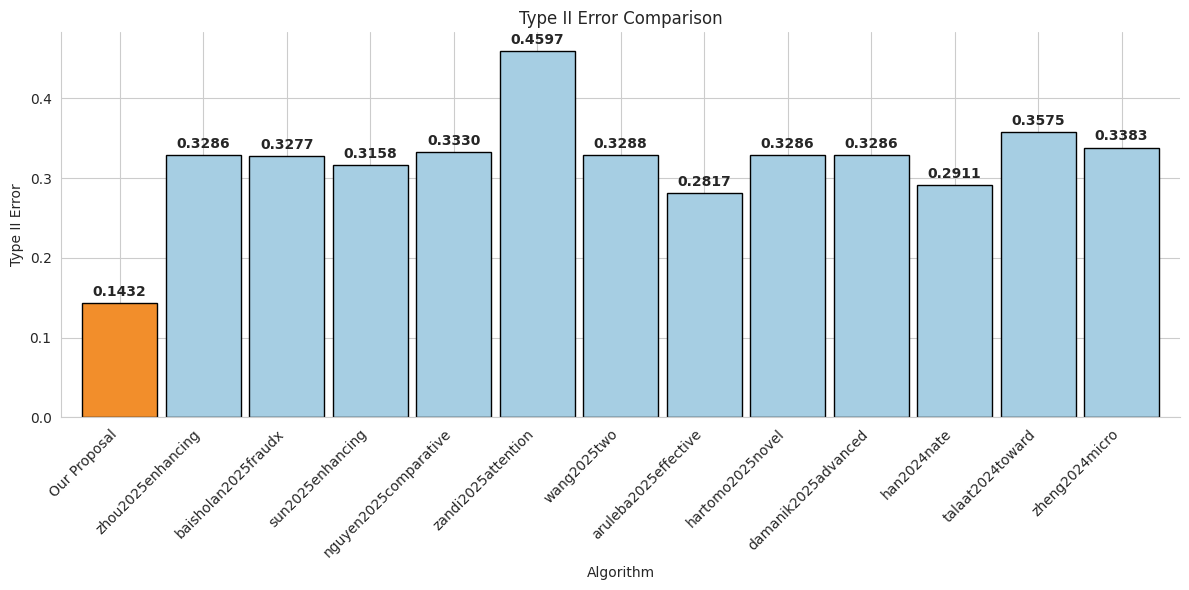
\includegraphics[width=0.95\linewidth]{img/errortipoII}
	\caption{Mean Type~II Error obtained by PbCRPE and the compared state-of-the-art approaches across the twelve evaluated credit risk datasets. Lower values indicate better prediction quality.}
	\label{fig:type2}
\end{figure}

Across the twelve evaluated datasets, PbCRPE achieves a mean AUC of \textbf{0.8566} and a mean Type~II Error of \textbf{0.1432}. The AUC results indicate that PbCRPE provides competitive prediction quality compared with the selected state-of-the-art approaches. In particular, PbCRPE attains the highest AUC on several datasets while maintaining competitive results on the remaining datasets. In terms of Type~II Error, PbCRPE achieves the best overall result among the evaluated approaches, indicating a lower proportion of actual defaulters incorrectly classified as non-defaulters.\newline

To further assess the statistical significance of the observed differences, the Friedman test was applied separately to the AUC and Type~II Error results across the twelve evaluated datasets. This non-parametric test evaluates whether statistically significant differences exist among the compared approaches based on their ranks across datasets. For both metrics, the best-performing approach within each dataset was assigned rank~1, with higher rank values corresponding to lower prediction quality. Consequently, lower average ranks indicate better overall prediction quality across the evaluated datasets. The corresponding Friedman test results are presented in Figures~\ref{fig:friedman_auc} and~\ref{fig:friedman_type2}.

\begin{figure}[H]
	\centering
	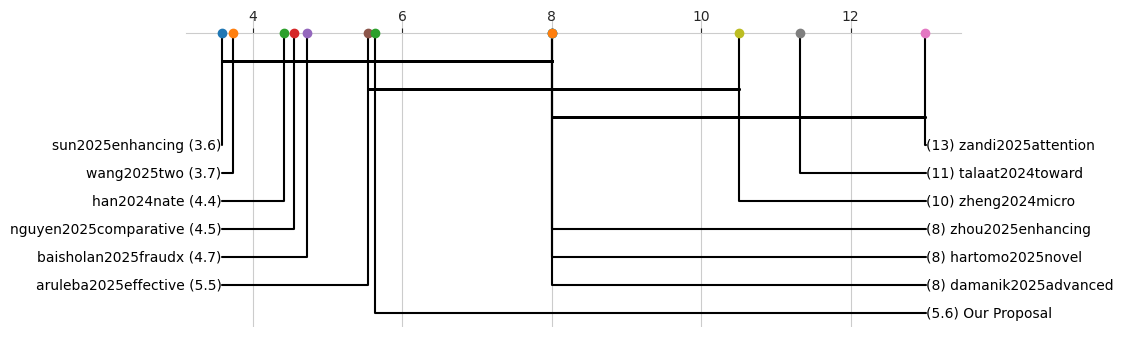
\includegraphics[width=0.95\linewidth]{img/friedman_auc}
	\caption{Friedman test results for AUC across the twelve evaluated credit risk datasets.}
	\label{fig:friedman_auc}
\end{figure}

\begin{figure}[H]
	\centering
	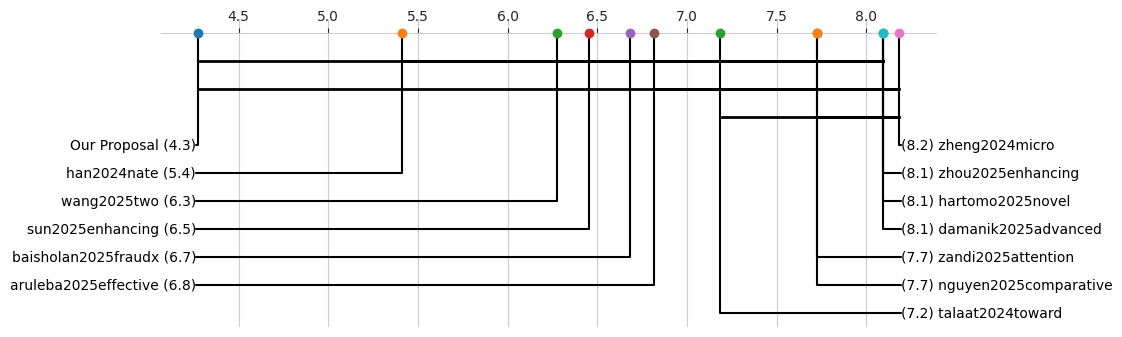
\includegraphics[width=0.95\linewidth]{img/friedman_typeiierror}
	\caption{Friedman test results for Type~II Error across the twelve evaluated credit risk datasets.}
	\label{fig:friedman_type2}
\end{figure}

For AUC, the statistical analysis indicates that PbCRPE remains competitive with the state-of-the-art works, as reflected by its relative ranking across the evaluated datasets. Although PbCRPE does not necessarily outperform all compared approaches in terms of AUC, its overall ranking demonstrates that its prediction quality is comparable to that of recent works reported in the literature.\newline

While the AUC results show that PbCRPE provides competitive prediction quality compared with the evaluated works, the Type~II Error results show that PbCRPE achieves the best overall result among the evaluated works. The proposed algorithm obtains the lowest mean Type~II Error and the best mean rank for this metric across the evaluated datasets. This result is particularly relevant from a practical credit risk perspective because Type~II Error measures the proportion of actual defaulters incorrectly classified as non-defaulters. A lower value therefore indicates a greater ability to identify customers who are likely to default, reducing the risk of incorrectly considering them as non-defaulters.\newline

To determine which pairwise differences between works are statistically significant, a Nemenyi post-hoc test was performed following the Friedman analysis. The resulting comparisons provide additional evidence regarding the relative position of PbCRPE with respect to the evaluated state-of-the-art works. For AUC, the post-hoc analysis shows that PbCRPE remains within the group of competitive works, with no statistically significant disadvantage with respect to the evaluated works. For Type~II Error, PbCRPE obtains the lowest mean rank, consistent with its lowest mean Type~II Error across the evaluated datasets. These results indicate that the proposed algorithm achieves the best overall position for this metric while maintaining competitive AUC results.\newline

From a practical perspective, the results obtained for Type~II Error are particularly important in credit risk prediction because failing to identify a defaulter may result in direct financial losses for lending institutions. Therefore, the low Type~II Error obtained by PbCRPE reflects its ability to reduce the proportion of actual defaulters incorrectly classified as non-defaulters. This result is particularly relevant because PbCRPE achieves the lowest Type~II Error while maintaining competitive overall discrimination capability in terms of AUC. Taken together, these results indicate that PbCRPE provides competitive prediction quality compared with recent state-of-the-art works while achieving the best overall results in terms of Type~II Error.


%\subsection{Explanation Analysis}\label{sec:explanation-analysis}
%The explanation analysis evaluates whether the contrast pattern mining algorithm provides sufficient pattern coverage for the instances evaluated by PbCRPE. In particular, we verify whether, for each evaluated instance $x$, at least one contrast pattern mined from a cluster associated with the predicted class covers $x$. This analysis directly evaluates the coverage assumption defined for the prediction and explanation stages. A prediction is considered covered when $\mathcal{P}*{c,j}(x) \neq \emptyset$ for at least one cluster $C*{c,j}$ associated with the predicted class $c$.\newline

%Across the twelve evaluated credit risk datasets, all evaluated instances were covered by at least one contrast pattern mined from a cluster associated with the predicted class. Consequently, the explanation stage successfully identified a covering contrast pattern for every evaluated prediction, and no fallback mechanism was required. This result provides empirical evidence that the proposed clustering and contrast pattern mining approach provides complete pattern coverage across the evaluated datasets.\newline

%Although this observation does not constitute a theoretical guarantee that every possible future instance will be covered, it confirms the empirical validity of the coverage assumption under the experimental conditions considered in this study.

\subsection{Discussion}

PbCRPE achieves competitive prediction quality compared with the twelve evaluated state-of-the-art works while simultaneously providing an explanation for each prediction. This dual capability, integrating prediction and explanation within a single algorithm, represents an important advantage over post-hoc explanation techniques such as SHAP and LIME, which typically express explanations through feature-level contribution or importance scores rather than explicitly representing a conjunction of feature-value conditions. This distinction is particularly relevant in credit risk prediction, where default risk is generally associated with combinations of financial and personal attributes rather than individual features considered in isolation~\cite{aruleba2025improved}.\newline

A key contribution of PbCRPE is therefore the representation of explanations as contrast patterns rather than as independent feature-importance scores. While SHAP assigns a contribution value to each feature according to its contribution to the prediction, and LIME estimates the local importance of features using an interpretable surrogate model, PbCRPE provides an explicit conjunction of $feature\#value$ conditions that jointly characterizes the prediction. Consequently, the explanation not only identifies which features are involved in the prediction, but also specifies the particular combination of conditions shared by the new instance and multiple similar instances within the selected cluster. For example, a pattern such as $\mathit{credit\_history} \neq \texttt{A34} \wedge \mathit{amount} < \$7{,}824 \wedge \mathit{duration} > 28\,\mathrm{months} \wedge \mathit{installment\_rate} > 2\% \wedge \mathit{num\_loans} \leq 1$ represents a joint configuration of conditions rather than a set of independent feature contributions. This representation preserves the relationships among the conditions and provides an explanation associated with a group of similar instances rather than with isolated feature contributions.\newline

This difference should not be interpreted as indicating that SHAP or LIME cannot account for feature interactions. Rather, the distinction lies in how the resulting explanation is represented. SHAP and LIME primarily summarize the local contribution or importance of individual features, whereas PbCRPE explicitly expresses the explanation as a conjunction of conditions that jointly cover the instance and are shared by similar instances. Therefore, PbCRPE provides a pattern-based representation that can be directly interpreted as a combination of $feature\#value$ conditions associated with the predicted class.\newline

To illustrate the explanation process, Table~\ref{tab:example_instance} presents an example of an instance from the German credit dataset that was classified by PbCRPE as \textit{defaulter}.\newline

\begin{table}[H]
	\centering
	\caption{Example instance from the German credit dataset.}
	\label{tab:example_instance}
	\renewcommand{\arraystretch}{1.15}
	\begin{tabularx}{\textwidth}{
			>{\raggedright\arraybackslash}p{0.19\textwidth}
			>{\centering\arraybackslash}p{0.08\textwidth}
			>{\centering\arraybackslash}p{0.12\textwidth}
			X
		}
		\toprule
		\textbf{Feature} & \textbf{Type} & \textbf{Value} & \textbf{Description} \\
		\midrule
		
		\textit{estatus\_cuenta} 
		& C 
		& A14 
		& No checking account \\
		
		\textit{duracion} 
		& N 
		& 36 
		& Duration of the credit: 36 months \\
		
		\textit{historial\_creditos} 
		& C 
		& A30 
		& No credits taken/all credits paid back duly \\
		
		\textit{finalidad} 
		& C 
		& A43 
		& Radio/television \\
		
		\textit{monto\_credito} 
		& N 
		& 3342 
		& Credit amount: \$3,342 \\
		
		\textit{cuenta\_ahorro} 
		& C 
		& A65 
		& Unknown/no savings account \\
		
		\textit{empleo\_actual} 
		& C 
		& A75 
		& Present employment for 7 years or more \\
		
		\textit{tasa\_interes} 
		& N 
		& 4 
		& Installment rate: 4\% of disposable income \\
		
		\textit{genero\_estadocivil} 
		& C 
		& A93 
		& Male, single \\
		
		\textit{aval} 
		& C 
		& A101 
		& No other debtors or guarantors \\
		
		\textit{residencia} 
		& N 
		& 2 
		& Present residence since 2 years \\
		
		\textit{propiedad} 
		& C 
		& A123 
		& Car or other property, excluding real estate and savings agreements/life insurance \\
		
		\textit{edad} 
		& N 
		& 51 
		& Age: 51 years \\
		
		\textit{planesdepago} 
		& C 
		& A143 
		& No other installment plans \\
		
		\textit{vivienda} 
		& C 
		& A152 
		& Own housing \\
		
		\textit{numero\_creditos} 
		& N 
		& 1 
		& One existing credit at this bank \\
		
		\textit{empleo} 
		& C 
		& A173 
		& Skilled employee/official \\
		
		\textit{dependientes} 
		& N 
		& 1 
		& One person liable to receive maintenance \\
		
		\textit{telefono} 
		& C 
		& A192 
		& Telephone registered under the customer's name \\
		
		\textit{trabajo\_extranjero} 
		& C 
		& A201 
		& Foreign worker: yes \\
		
		\bottomrule
	\end{tabularx}
\end{table}

For the instance shown in Table~\ref{tab:example_instance}, PbCRPE first considers the clusters associated with the predicted class. Using the contrast pattern-based similarity score defined in Equation~\ref{eq:cluster_similarity}, the cluster with the highest similarity to the new instance is selected. Subsequently, among the contrast patterns from the selected cluster that cover the new instance, the pattern with the highest support is selected according to the criterion defined in Equation~\ref{eq:pattern_selection}:

\[
\begin{aligned}
	&\mathit{credit\_history} \neq \texttt{A34} \wedge
	\mathit{amount} < \$7{,}824 \wedge
	\mathit{duration} > 28\,\mathrm{months} \\
	&\wedge\ 
	\mathit{installment\_rate} > 2\% \wedge
	\mathit{num\_loans} \leq 1
\end{aligned}
\]

Thus, the selected contrast pattern covers the instance because all of its $feature\#value$ conditions are simultaneously satisfied. For example, the condition $\mathit{credit\_history} \neq \texttt{A34}$ is satisfied because the instance has an \textit{No credits taken/all credits paid back duly} credit history, which corresponds to a value different from \texttt{A34}. Similarly, $\mathit{amount} < \$7{,}824$ is satisfied because the credit amount is \$3,342; $\mathit{duration} > 28\,\mathrm{months}$ is satisfied because the duration is 36 months; $\mathit{installment\_rate} > 2\%$ is satisfied because the installment rate is 4\%; and $\mathit{num\_loans} \leq 1$ is satisfied because the instance has one existing loan. Since a contrast pattern is defined as a conjunction of conditions, all these conditions must be satisfied simultaneously for the pattern to cover the instance. Importantly, the pattern is not interpreted as a collection of independent feature contributions. Rather, its conjunction represents a combination of $feature\#value$ conditions shared by the new instance and multiple similar instances within the selected cluster. Consequently, the contrast pattern provides a concise representation of the combination of conditions associated with the predicted credit risk class.\newline

The example also illustrates the role of performing contrast pattern mining at the cluster level rather than directly at the class level. Instead of extracting patterns intended to represent all instances belonging to the same class, PbCRPE mines contrast patterns from groups of similar instances. This strategy allows different local structures within the same class to be captured, enabling the resulting patterns to represent $feature\#value$ conditions that are more specific to particular groups of similar instances. Therefore, the resulting explanations are associated not only with the predicted class but also with a specific group of similar instances represented by the selected cluster.\newline

The experimental results confirm that the coverage condition required by the explanation procedure was satisfied for all evaluated instances. In particular, for every evaluated instance across all twelve datasets, at least one contrast pattern mined from a cluster associated with the predicted class covered the instance. Therefore, the similarity score could be computed from covering contrast patterns for all evaluated instances, and the explanation procedure could be applied without requiring any fallback mechanism. These results provide empirical evidence that the coverage condition defined in the explanation procedure was consistently satisfied under the experimental conditions considered in this study.\newline

Taken together, these results indicate that PbCRPE combines competitive prediction quality with explanations based on contrast patterns that represent combinations of $feature\#value$ conditions shared by similar instances. By integrating prediction for mixed-type and imbalanced data with cluster-level contrast pattern mining and representative pattern selection, PbCRPE generates explanations that are directly associated with groups of similar instances rather than isolated feature contributions. These results support the applicability of the proposed algorithm to credit risk datasets involving mixed-type features and class imbalance, where both prediction quality and explainable decision support are relevant.
}
	\printbibliography
\end{document}
